%%%%%%%%%%%%%%%%%%%%%%%%%%%%%%%%%%%%%%%%%%%%%%%%%%%%%%%%%%%%%%%%%%%%%%
%% Fconclusion.tex
%% Description:   
%% Author:        Carsten Wulff <wulff@iet.ntnu.no>
%% Created at:    Thu Apr 24 16:46:39 2008
%% Modified at:   Wed Oct 29 19:41:13 2008
%% Modified by:   Carsten Wulff <wulff@iet.ntnu.no>
%%%%%%%%%%%%%%%%%%%%%%%%%%%%%%%%%%%%%%%%%%%%%%%%%%%%%%%%%%%%%%%%%%%%%%
\chapter{Comments to papers, conclusion and further work}\label{sc:remarks}


\section{Comments to papers}
\subsection{Paper 2}
In the suggested future work of this paper we mention that an integrated circuit
implementation would be the next step. We did investigate some
implementations on the simulation level, but we discovered that low-pass noise
shaping was insufficient to create an efficient high-speed,
high-resolution ADC. With a high oversampling ratio in a high-speed modulator the requirements
for the unity gain of the opamps was to high. Thus, we decided to
concentrate on more aggressive noise shaping using zeros at non-zero
frequency to lower the OSR of the modulator. 

\subsection{Paper 4}
The comparator developed in this paper was intended for the
pipelined ADCs in this thesis (Paper 5 and Paper 7), but a problem was
discovered after publication. The comparator in Paper 4 has
significant kick-back through the input transistors M1 and M4. In the 
reset phase the drain of these transistors are reset to ground. When the
comparator turns on, both the sources go to VDD. This results in a kick-back through the gate-source
capacitor. The kick-back can become large if
input capacitance of the comparator 
is significant compared to the sampling capacitors in the pipelined stage. As a consequence, 
this comparator was not used in Papers 5 and Paper 7.

\subsection{Paper 7}
Fig. \ref{fig:adccomp} shows a
comparison of this ADC to other 8-bit converters. At 8-bits and above
1MS/s there are three converters that have 
better FOM. The first is a zero-based
crossing switched-capacitor (similar to CBSC) by Brooks et al with
4.5fJ/step at 200MS/s
\cite{brooks07a}, this was a single ended architecture implemented in
0.18$\mu m$
CMOS. The second is by Kim et al \cite{kim05}  in a 0.18$\mu m$ CMOS
technology with a FOM of
3.56fJ/step at 200MS/s. They used switched-opamps to reduce power dissipation.
The third
is by Mulder et al \cite{mulder04} with 4.5fJ/step at 125MS/s, this was a
sub-ranging ADC in 0.13$\mu m$ CMOS technology. At 8-bit and above
1MS/s there is only one other ADC in 90nm CMOS by Shen et
al\cite{shen08}, which has a FOM of 11.37fJ/step at 10MS/s.

The ADC in Paper 7 was designed to be a 10-bit converter, but we
underestimated the noise from digital IO, which limited the
performance. Thus, the ADC was not optimized for 8-bit operation, and
in that light the achieved performance is satisfactory.


\begin{figure}[htb]
\centering 
 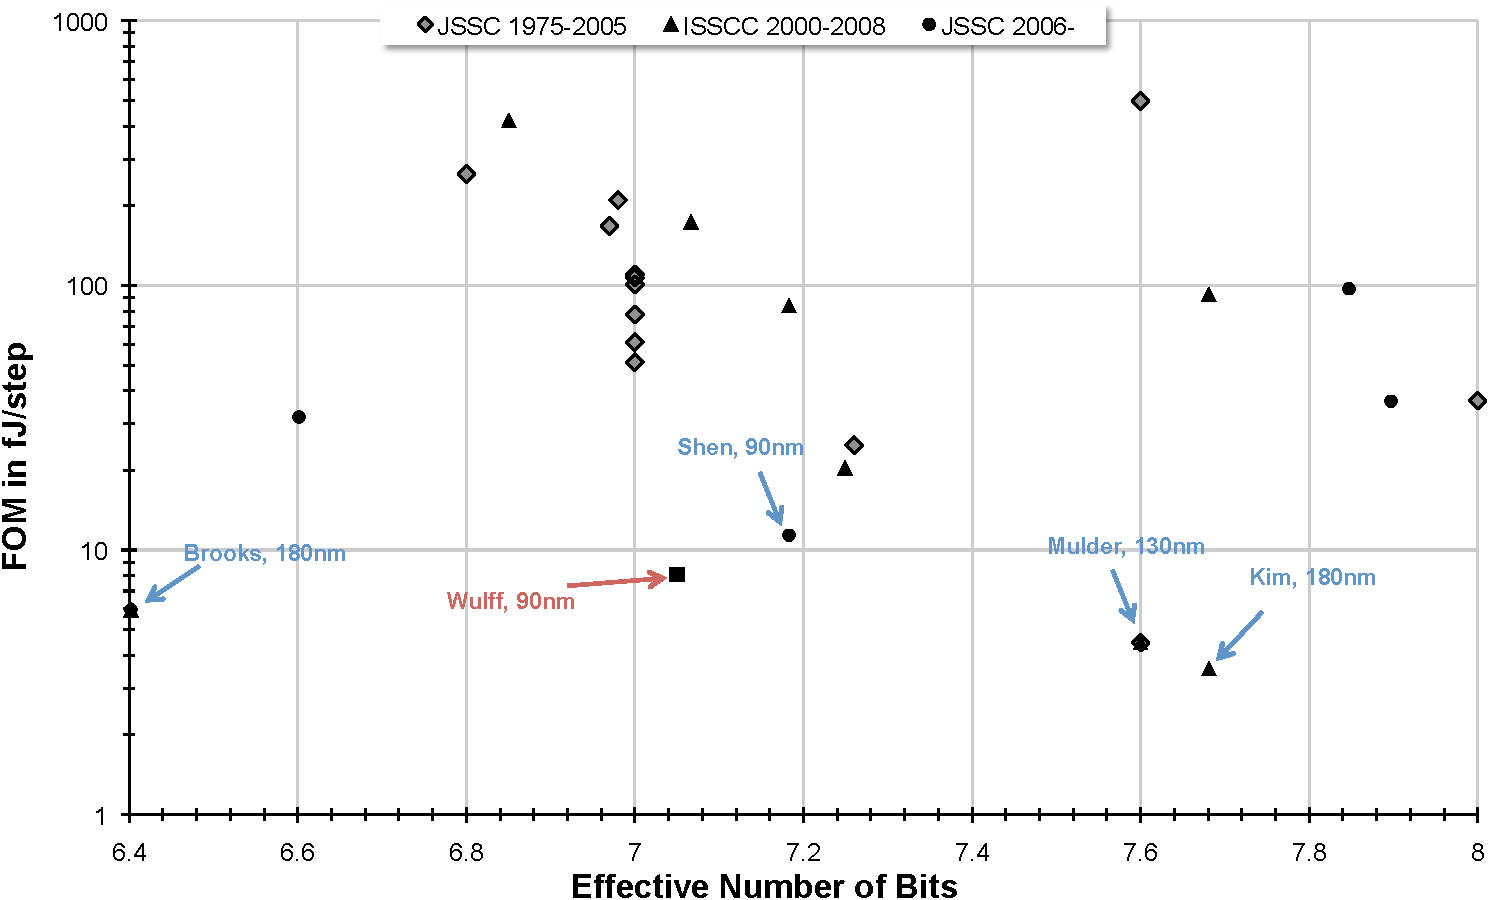
\includegraphics[width=\myfigwidth]{graphics/adccomp}
  \caption{Figure of merit comparison of the ADC in Paper 7 and other
    eight bit converters with sampling frequency above 1MS/s. A lower
    value is better.}
  \label{fig:adccomp}
\end{figure}

\section{Conclusion}
In this thesis we have focused on two of the challenges facing an ADC
designer in nano-scale CMOS technology, reduced power supply  and reduced
output resistance. 

For high-resolution ($ \ge 12$-bit) ADCs one
of the challenges is the increased capacitance due to reduced signal
swing. As seen in \reg{supplyscaling} the power supply is expected
to reach 0.65V at the 14nm node (year 2020). If we assume the signal swing
is 80\% of the power supply a 12-bit ADC will require a minimum of
12pF sampling capacitance, while a 14-bit ADC will require 192pF
sampling capacitance. Hence, high-resolution
converters in nano-scale CMOS must use oversampling to reduce the capacitance. 


The
switched-capacitor open-loop
sigma-delta modulator introduced in this work is a new architecture. In this thesis we have described how one can build such an ADC
and explained most of the theory behind OLSDM.  We believe that OLSDM
is an interesting alternative to the
MASH\footnote{MASH: Multi-stAge noise SHaping} sigma-delta as a
front-end 
to pipelined ADCs.

Another challenge for pipelined ADCs and sigma-delta ADCs is reduced headroom and reduced output resistance. The
reduced headroom makes it harder to stack transistors (cascoding) to
achieve high gain. This combined with the reduced output 
resistance of nano-scale CMOS transistors make it difficult to design
high gain circuits. Unless something is done at the device level it
will be challenging to design high gain ($>$ 40dB) operational
amplifiers in the future nano-scale CMOS technologies. 

For high-resolution ($\ge 12$-bit) high-speed ADCs techniques like
correlated-level shifting \cite{gregoire08} or gain-calibration \cite{mcneill05} could be alternatives
to conventional opamps. 

For low- to medium-resolution (6-bit to 10-bit) high-speed ADCs techniques like open-loop residue amplifiers and comparator-based
switched-capacitor circuits are an alternative to opamp-based SC. 

 For pipelined ADCs up to 7-bit the open-loop residue
amplifier is a good option, as was demonstrated in Paper 5. But the use
of open-loop residue amplifiers above 7-bit requires calibration due to
the non-linearity of open-loop amplifiers. 

Comparator-based switched-capacitor ADCs can bridge the gap from 7-bit to 10-bit resolution.  We have
shown that it is possible to create a differential CBSC ADC. And we
have shown that the efficiency of such a converter is
good. The ADC in Paper 7 is only two times less efficient than the best 8-bit ADCs
above 1MS/s. To par the best ADCs it would have to increase
its resolution by 0.5-bit (from
7.05-bit to 7.5-bit). As the pipelined ADC in Paper 7 was designed for
10-bit operation and achieved 9-bit ENOB in simulation we believe that
differential CBSC pipelined ADCs can be made more efficient than our prototype. The limiting factor
in our ADC was noise from digital IO, which is an problem that can be
solved. 
%The speed of the digital IO limited the speed of the
%converter. 

\section{Further work}


For open-loop sigma-delta modulation the next question is:
What is the expression for the  effect of incomplete settling in the modulo resonator and
the modulo integrator? The effects of incomplete settling are well
known for conventional integrators, but it must be verified that the
modulo operation does not introduce any new phenomena. An analytical expression that can be translated
into a MATLAB model is needed, and it should be verified with SPICE
simulations. A place to start is with the papers by Temes \cite{temes80}
and Martin \cite{martin81}, which detail the effects of incomplete settling for
switched-capacitor integrators. 


For comparator-based switched capacitor ADCs there are two challenges we
would like to mention. 
Our ADC has digitally controlled current sources and comparators and a
digital calibration algorithm is used to calibrate the ADC. But the search
space is too large, $2^{154}-1$ is simply too many possible solutions. In
future versions we would recommend limiting the search space. One way to
do this is to reduce the number of CBSC stages. We believe that a
combination of MSB CBSC stages and LSB opamp-based stages, LSB open-loop
residue amplifier stages, or a multi-bit flash-ADC is the way to go. For
example a 10-bit pipelined ADC with four CBSC stages and a 6-bit
back-end. The search space for calibration of CBSC
stages is then reduced. With our calibration method there would be
$2^{88}-1$ possible solution,
which still is too many. But with the help of the design equations in
Paper 6 the search space can be further reduced. The necessary
comparator threshold ($V_{ct}$) can be calculated from the comparator delay ($T_d$), the
current source current ($I_0$), the output capacitance ($C_o$) and the
output resistance ($R_o$). With SPICE simulations the standard deviation of
these variables can be found. Accordingly, the standard deviation of $V_{ct}$
could be found, which would limit the number of bits required to
calibrate it after production.


Another challenge is the noise from digital IO. For future prototypes
we would recommend synchronizing all bits. Knowing when the digital
outputs switch is essential. Reducing the number of bits would also
be a good idea. For a pipelined ADC with four CBSC stages and a 6-bit back-end we would
need $2\times4 + 6
= 14$ digital outputs, compared to 18 digital outputs for eight CBSC stages and a two
bit flash-ADC. In addition, in an ADC prototype is a good idea to include a down-sampler, so the digital
outputs can be run at a lower speed than the ADC core. We did not do
this for the ADC in Paper 7, but we wish we had. 







%%% Local Variables: 
%%% mode: latex
%%% TeX-master: "tb_conclusion"
%%% End: 
